%!TEX program = xelatex

\documentclass[12pt]{beamer}
\usepackage{graphicx}

\setlength{\parindent}{0pt}

%\setbeameroption{show notes}
\makeatletter
\def\beamer@framenotesbegin{% at beginning of slide
    \gdef\beamer@noteitems{}%
    \gdef\beamer@notes{{}}% used to be totally empty.
}
\makeatother

% Theme stuff
% -----------
\usetheme{default}
\beamertemplatenavigationsymbolsempty
%\setbeamertemplate{itemize item}[circle]
\setbeamertemplate{itemize items}{$\bullet$}
\setbeamertemplate{itemize subitem}{$\circ$}
\setbeamercolor{itemize item}{fg=black}
\setbeamercolor{itemize subitem}{fg=black}
\setbeamercolor{itemize subsubitem}{fg=black}
\setbeamertemplate{enumerate items}[default]
\setbeamercolor{enumerate item}{fg=black}
\setbeamercolor{enumerate subitem}{fg=black}
%\setbeamertemplate{footline}[frame number]

% Algorithm stuff
% ---------------
\usepackage[vlined,linesnumbered]{algorithm2e}
\newcommand\mycommfont[1]{\textcolor{gray}{#1}}
\SetCommentSty{mycommfont}

% Font stuff
% ----------
\usepackage[no-math]{fontspec}
\defaultfontfeatures{Mapping=tex-text}
\setsansfont[BoldFont=P22UndergroundBook,
			 SmallCapsFont=P22UndergroundLightSC]{P22UndergroundLight}
\setmonofont{Hack}



% Define colors
% -------------
\usepackage{xcolor}
\definecolor{BGDarkGrey}{RGB}{50,50,50}
\definecolor{BGBlue}{RGB}{77,143,249}
\definecolor{LightGrey}{RGB}{200,200,200}
\definecolor{Grey50}{RGB}{128,128,128}
\definecolor{LBlue}{HTML}{29B6F6}
\definecolor{Blue}{HTML}{42A5F5}
\definecolor{Orange}{HTML}{FFA726}
\definecolor{LGreen}{HTML}{9CCC65}
\definecolor{Green}{HTML}{66BB6A}
\definecolor{Red}{HTML}{EF5350}
\definecolor{Amber}{HTML}{FFCA28}
\definecolor{Yellow}{HTML}{FFEE58}
\definecolor{Cyan}{HTML}{26C6DA}
\definecolor{Indigo}{HTML}{5C6BC0}
\definecolor{Lime}{HTML}{D4E157}
\definecolor{BlueGrey}{HTML}{78909C}
\definecolor{DeepOrange}{HTML}{FF7043}
\definecolor{Grey}{HTML}{424242}
\definecolor{Teal}{HTML}{26A69A}
\definecolor{PaleYellow}{RGB}{255,255,153}

\definecolor{DhakaBlue}{RGB}{102,167,221}
\definecolor{WikiGrey}{RGB}{252,252,252}

\renewcommand{\arraystretch}{2}

% Table package
% -------------
\usepackage{booktabs}

% Background
% ----------
\usepackage{tikz}

\begin{document}


% Title
\setbeamercolor{normal text}{fg=Grey, bg=white}
\usebeamercolor[fg]{normal text}
\begin{frame}

	\null
	\vfill
	%\centering
	\textcolor{black}{\textsc{\large A Comparative Study of Techniques for Estimation and Inference of Nonlinear Stochastic Time Series}} \\
	\vspace{1.5\baselineskip}
	\noindent\textcolor{black}{\rule{\textwidth}{0.4pt}} \\
	\vspace{2\baselineskip}
	Dexter Barrows, B.Sc. \\
	\vspace{1\baselineskip}
	Masters Thesis Defence \\
	McMaster University \\
	April 2016
	\vfill

\end{frame}


% Authors
\setbeamercolor{normal text}{fg=Grey, bg=white}
\usebeamercolor[fg]{normal text}
\begin{frame}

	\vspace{\baselineskip}
	\begin{columns}
		\begin{column}{0.8\textwidth}
			{\large
			\begin{enumerate}
				\item Framing
				\item Stochastic SIR Model
				\item Hamiltonian HMCMC
				\item Iterated Filtering 2
				\item Forecasting Frameworks
				\item S-maps \& Seasonal Outbreaks
				\item Spatiotemporal Epidemics
				\item Parallelism \& Future Directions
			\end{enumerate}
			}
		\end{column}
	\end{columns}

\end{frame}

%% 1. INTRODUCTION
%% --------------------------------------------------------------------------------------
%% --------------------------------------------------------------------------------------

% Section title
\setbeamercolor{normal text}{fg=white, bg=BGBlue}
\usebeamercolor[fg]{normal text}
\begin{frame}

	\vspace{2cm}
	\hspace{2.5cm} {\Huge Framing }
	\begin{tikzpicture}[overlay]
	    \node[at=(current page.center), shift={(-4.5 cm, -4.7 cm)}, opacity=0.25] {
	    	\fontsize{200pt}{0pt}\selectfont
	        \color{white}{1}
	    };
	\end{tikzpicture}

\end{frame}

\setbeamercolor{normal text}{fg=Grey, bg=white}
\usebeamercolor[fg]{normal text}
\begin{frame}

	\null
	\vfill
	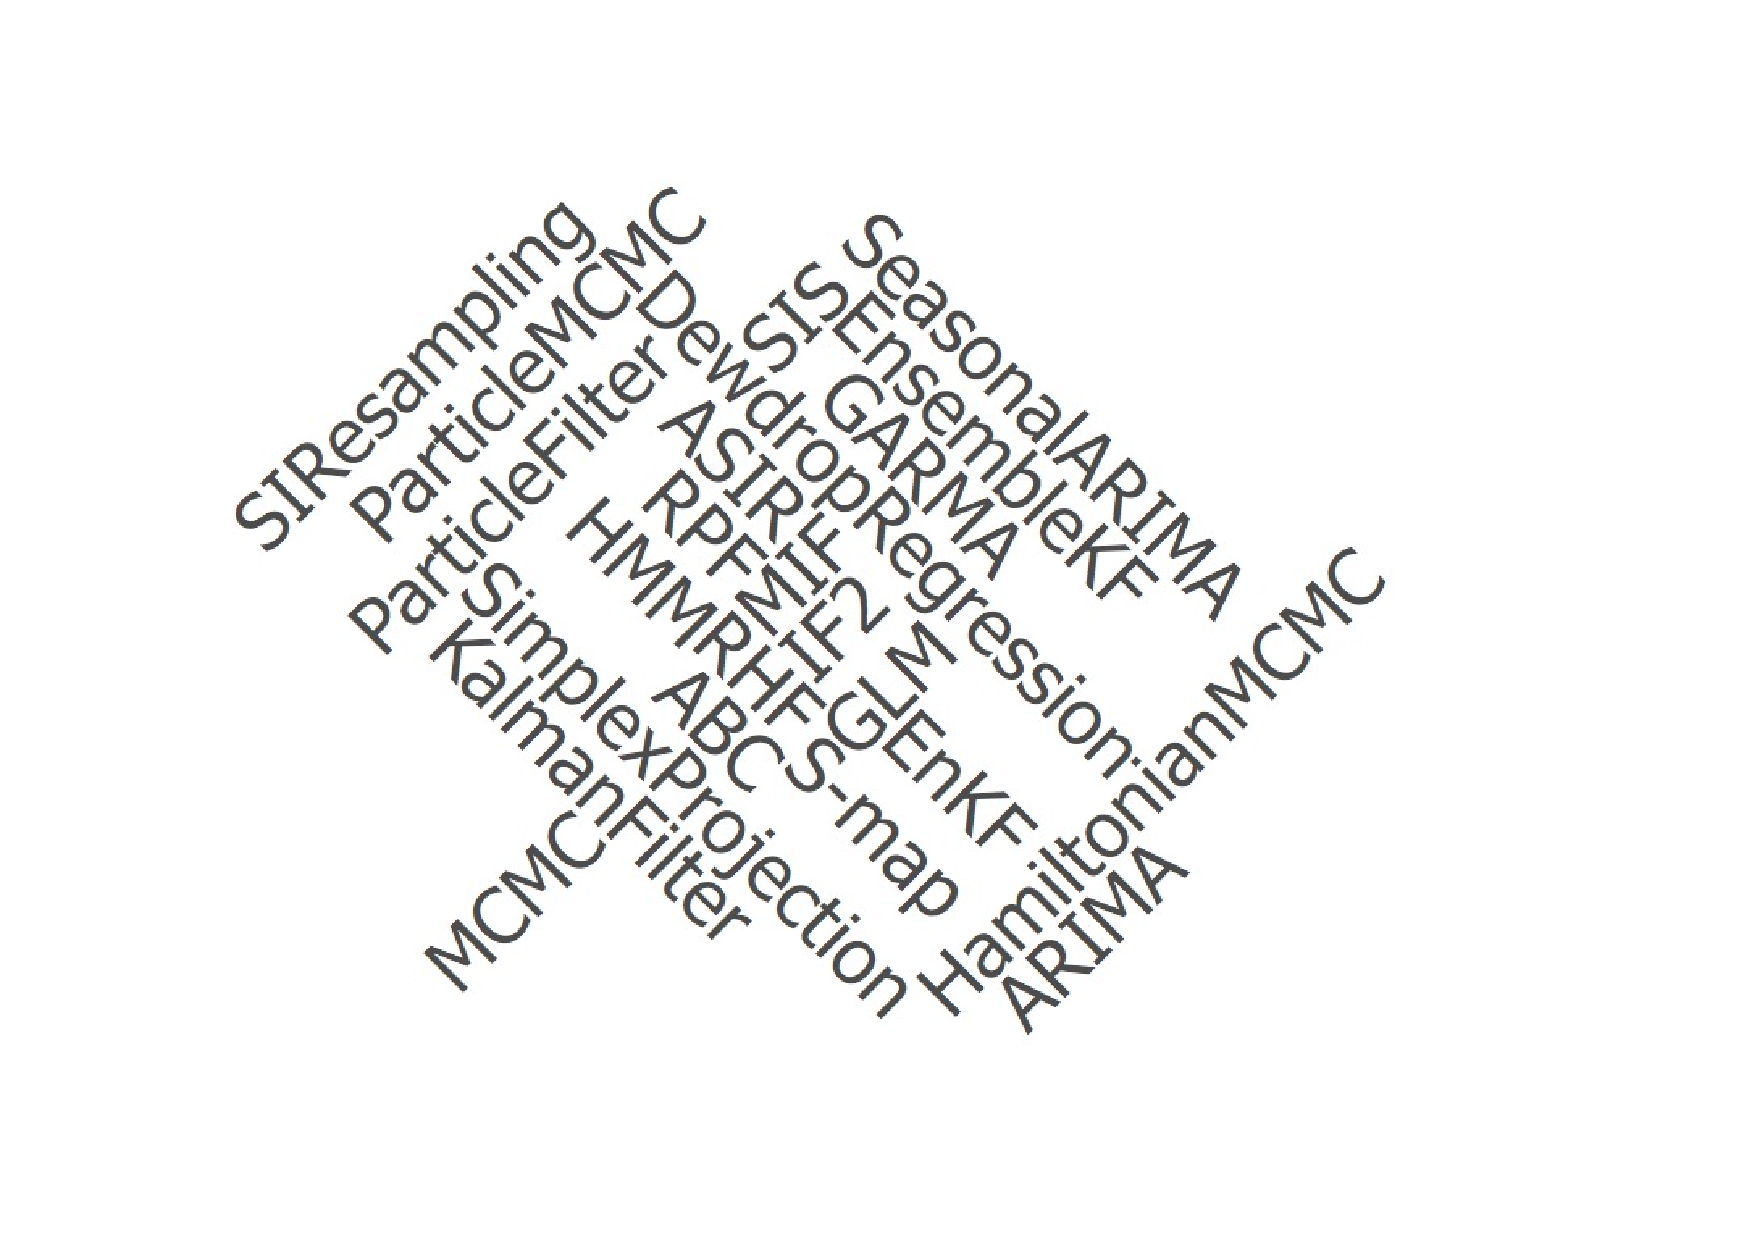
\includegraphics[width=\textwidth,height=\textheight,keepaspectratio=true]{images/wordcloud}
	\vfill

\end{frame}


%% 2. Stochastic SIR model
%% --------------------------------------------------------------------------------------
%% --------------------------------------------------------------------------------------

% Section title
\setbeamercolor{normal text}{fg=white, bg=Amber}
\usebeamercolor[fg]{normal text}
\begin{frame}

	\vspace{2cm}
	\hspace{0cm} {\Huge Stochastic SIR Model } \\
	\begin{tikzpicture}[overlay]
	    \node[at=(current page.center), shift={(3.2 cm, -4 cm)}, opacity=0.25] {
	    	\fontsize{200pt}{0pt}\selectfont
	        \color{white}{2}
	    };
	\end{tikzpicture}

\end{frame}

% Basic Stochastic SIR
\setbeamercolor{normal text}{fg=white, bg=Grey}
\setbeamercolor{footline}{parent=normal text}
\usebeamercolor[fg]{normal text}
\begin{frame}

	\null
	{\large \textcolor{Cyan}{Stochastic SIR model}}
	\vfill

	\centering
	\begin{align*}
		\dfrac{dS}{dt} 	& = - \beta S I \\
		\dfrac{dI}{dt} 	& = \beta S I - \gamma I \\
		\dfrac{dR}{dt} 	& =  \gamma I
	\end{align*}
	\vspace{0.5\baselineskip}
	$+$	\\
	\vspace{1\baselineskip}
	$\beta_{t+1} = \exp \left[ \beta_t + \eta \left( \bar{\beta} - \beta_t \right) + \mathcal{N}(0, \sigma_{\small\text{proc}}) \right]$

\end{frame}

\setbeamercolor{normal text}{fg=Grey, bg=white}
\usebeamercolor[fg]{normal text}
\begin{frame}

	\null
	\vfill
	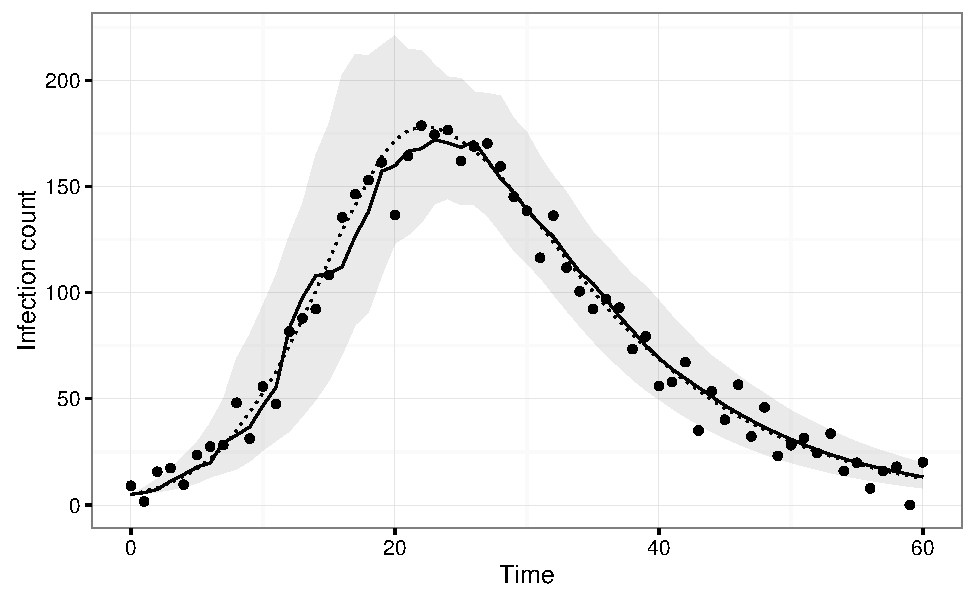
\includegraphics[width=\textwidth,height=\textheight,keepaspectratio=true]{../../writing/SC1/images/sirmean}
	\vfill

\end{frame}


%% 3. HMCMC
%% --------------------------------------------------------------------------------------
%% --------------------------------------------------------------------------------------

% Section title
\setbeamercolor{normal text}{fg=white, bg=Green}
\usebeamercolor[fg]{normal text}
\begin{frame}

	\vspace{2cm}
	\hspace{0cm} {\Huge Hamiltonian MCMC }
	\begin{tikzpicture}[overlay]
	    \node[at=(current page.center), shift={(-5.2 cm, -4.7 cm)}, opacity=0.25] {
	    	\fontsize{200pt}{0pt}\selectfont
	        \color{white}{3}
	    };
	\end{tikzpicture}

\end{frame}

\setbeamercolor{normal text}{fg=Grey, bg=white}
\usebeamercolor[fg]{normal text}
\begin{frame}

	\begin{columns}
		\begin{column}{0.5\textwidth}

			\large
			MCMC
			\vspace{\baselineskip}

			\normalsize
			Iteratively construct Markov chain to approximate posterior

			\vspace{\baselineskip}

			\footnotesize
			\begin{enumerate}
				\item Choose starting parameter set
				\item Generate N samples by
				\begin{enumerate}
					\footnotesize
					\item Propose new sample
					\item Compute acceptance ratio
					\item Accept/reject sample
				\end{enumerate}
			\end{enumerate}
			
		\end{column}
		\begin{column}{0.5\textwidth}

			\tiny
			\begin{algorithm}[H]

		        \BlankLine

		        \SetKwInOut{Input}{Input}
		        \SetKwInOut{Output}{Output}
		        \DontPrintSemicolon

		        \tcc{Select a starting point}
		        \Input{Initialize $\theta^{(1)}$}

		        \BlankLine

		        \For{$i = 2:N$}{

		            \BlankLine

		            \tcc{Sample}
		            $\theta^* \sim q(\cdot|\theta^{(i-1)})$ \;
		            $u \sim \mathcal{U}(0,1)$

		            \BlankLine

		            \tcc{Evaluate acceptance ratio}
		            $r$ $\gets$ $\frac{\mathcal{L}(\theta^*)p(\theta^*)}{\mathcal{L}(\theta)p(\theta)}$

		            \BlankLine

		            \tcc{Step acceptance criterion}
		            \eIf{ $u < \min\left\{ 1 , r \right\}$ }{ 
		                $\theta^{(i)} = \theta^*$\;
		            }{
		                $\theta^{(i)} = \theta^{(i-1)}$\;
		            }
		        }

		        \BlankLine

		        \tcc{Samples from approximated posterior distribution}
		        \Output{Chain of samples $(\theta^{(1)},\theta^{(2)},...,\theta^{(N)})$}

		        \BlankLine

		        %\caption{Metropolis MCMC \label{mhmcmc}}

		    \end{algorithm}

		\end{column}
	\end{columns}

\end{frame}


\setbeamercolor{normal text}{fg=Grey, bg=white}
\usebeamercolor[fg]{normal text}
\begin{frame}
	
	\null
	{\large Hamiltonian Dynamics}
	\vspace{\baselineskip}
	\vfill

	\footnotesize

	\begin{align*}
		& \text{Energy} & & \\
		& \quad\quad \text{Kinetic} 	& K(r) 					& = \frac{1}{2} r^T M^{-1} r \\
		& \quad\quad \text{Potential} 	& U(\theta) 			& = - \log(\mathcal{L}(\theta)p(\theta)) \\
		& & & \\
		& & & \\
		& \text{Hamiltonian} 			& H(\theta,r)  			& = U(\theta) + K(r) \\
		& & & \\
		& & & \\
		& \text{Dynamics simulation}	& \frac{d\theta}{dt} 	& = M^{-1} r \\
		& 								& \frac{dr}{dt}			& = - \nabla U (\theta) \\
	\end{align*}

	\vfill

\end{frame}

\setbeamercolor{normal text}{fg=Grey, bg=white}
\usebeamercolor[fg]{normal text}
\begin{frame}

	\begin{columns}
		\begin{column}{0.6\textwidth}

			\large
			HMCMC algorithm
			\vspace{\baselineskip}

			\footnotesize
			\begin{enumerate}
				\item Choose starting parameter set
				\item Generate N samples by
				\begin{enumerate}
					\footnotesize
					\item Resampling moments
					\item Simulate Hamiltonian dynamics using Leapfrog integration
					\item Compute acceptance ratio
					\item Accept/reject sample
				\end{enumerate}
			\end{enumerate}
			
		\end{column}
		\begin{column}{0.4\textwidth}

			\tiny
			\begin{algorithm}[H]

		        \SetKwInOut{Input}{Input}
		        \SetKwInOut{Output}{Output}
		        \DontPrintSemicolon

		        \tcc{Select a starting point}
		        \Input{Initialize $\theta^{(1)}$}

		        \For{$i = 2:N$}{

		            \tcc{Resample moments}
		            \For{$i = 1:n$}{
		                r(i) $\gets$ $\mathcal{N}(0,1)$
		            }

		            \tcc{Leapfrog initialization}
		            $\theta_0$ $\gets$ $\theta^{(i-1)}$ \;
		            $r_0$ $\gets$ $r - \nabla U(\theta_0) \cdot \varepsilon / 2$

		            \tcc{Leapfrog intermediate steps}
		            \For{$j = 1:L-1$}{
		                $\theta_j$ $\gets$ $\theta_{j-1} + M^{-1} r_{j-1} \cdot \varepsilon$ \;
		                $r_j$ $\gets$ $r_{j-1} - \nabla U(\theta_j) \cdot \varepsilon$
		            }

		            \tcc{Leapfrog last steps}
		            $\theta^*$ $\gets$ $\theta_{L-1} + M^{-1} r_{L-1} \cdot \varepsilon$ \;
		            $r^*$ $\gets$ $\nabla U(\theta_L) \cdot \varepsilon / 2 - r_{L-1}$

		            \tcc{Evaluate acceptance ratio}
		            $r = \exp \left[ H(\theta^{(i-1)},r) - H(\theta^*,r^*) \right]$

		            \tcc{Sample}
		            $u \sim \mathcal{U}(0,1)$

		            \tcc{Step acceptance criterion}
		            \eIf{ $u < \min\left\{ 1 , r \right\}$ }{ 
		                $\theta^{(i)} = \theta^*$\;
		            }{
		                $\theta^{(i)} = \theta^{(i-1)}$\;
		            }
		        }

		        \tcc{Samples from approximated posterior distribution}
		        \Output{Chain of samples $(\theta^{(1)},\theta^{(2)},...,\theta^{(N)})$}

		    \end{algorithm}

		\end{column}
	\end{columns}

\end{frame}

\setbeamercolor{normal text}{fg=Grey, bg=white}
\usebeamercolor[fg]{normal text}
\begin{frame}

	\null
	\vfill
	HMCMC state reconstruction sample \\
	\vspace{\baselineskip}
	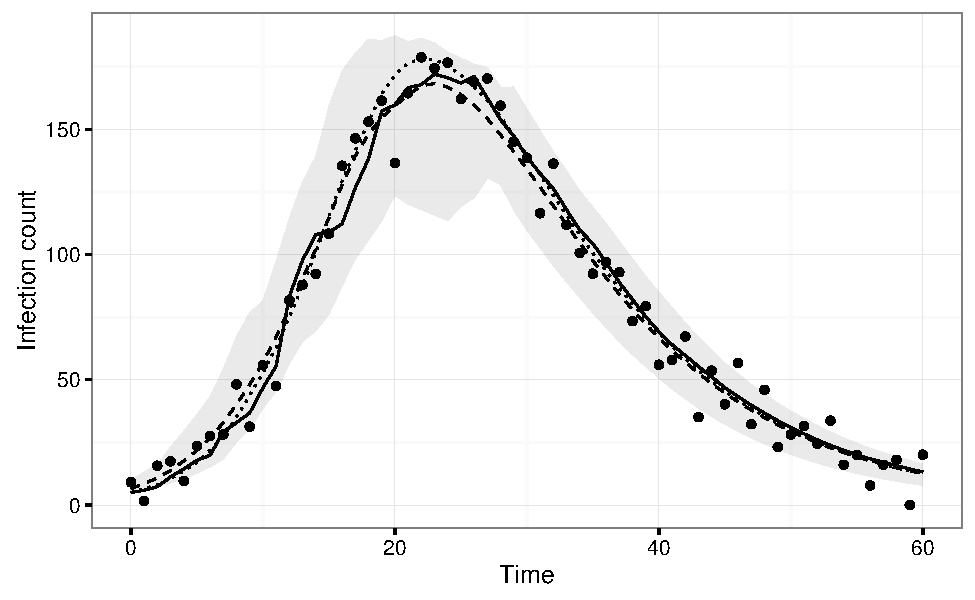
\includegraphics[width=\textwidth,height=\textheight,keepaspectratio=true]{../../writing/SC1/images/hmcboot}
	\vfill

\end{frame}

\setbeamercolor{normal text}{fg=Grey, bg=white}
\usebeamercolor[fg]{normal text}
\begin{frame}

	\null
	\vfill
	HMCMC parameter estimation kernels sample \\
	\vspace{\baselineskip}
	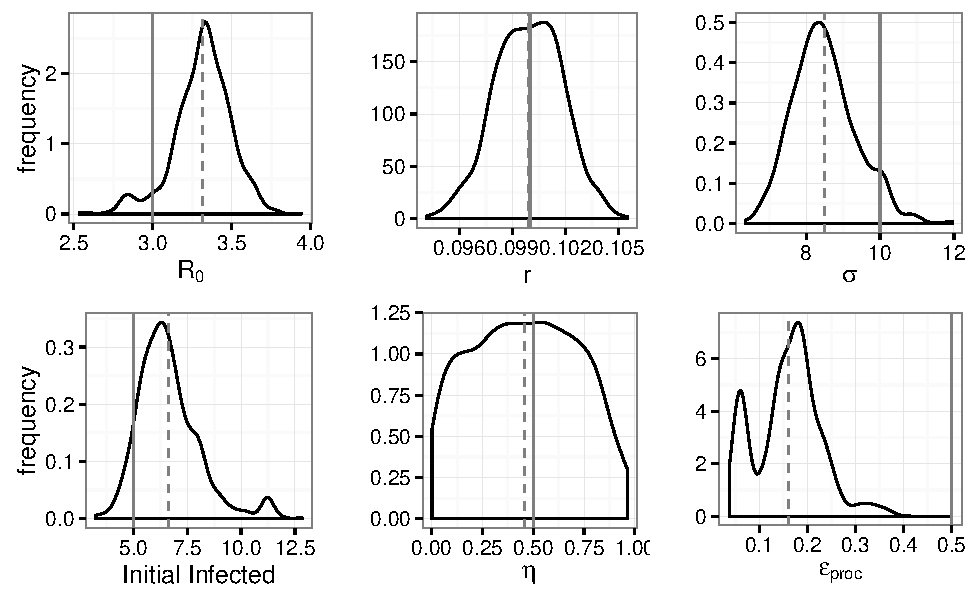
\includegraphics[width=\textwidth,height=\textheight,keepaspectratio=true]{../../writing/SC1/images/hmckernels}
	\vfill

\end{frame}


%% 4. IF2
%% --------------------------------------------------------------------------------------
%% --------------------------------------------------------------------------------------

% Section title
\setbeamercolor{normal text}{fg=white, bg=Red}
\usebeamercolor[fg]{normal text}
\begin{frame}

	\vspace{2cm}
	\hspace{0cm} {\Huge Iterated Filtering 2 }
	\begin{tikzpicture}[overlay]
	    \node[at=(current page.center), shift={(-4.7 cm, -4.7 cm)}, opacity=0.25] {
	    	\fontsize{200pt}{0pt}\selectfont
	        \color{white}{4}
	    };
	\end{tikzpicture}

\end{frame}

\setbeamercolor{normal text}{fg=Grey, bg=white}
\usebeamercolor[fg]{normal text}
\begin{frame}

	\begin{columns}
		\begin{column}{0.5\textwidth}

			\large
			Basic Particle Filter
			\vspace{\baselineskip}
			\footnotesize

			Iterative prediction-update cycle prunes particle cohort of poor parameter estimates

			\begin{enumerate}
				\item Initialize particles with parameter sets
				\item For each data point
				\begin{enumerate}
					\footnotesize
					\item Evolve particle states
					\item Weight via likelihood
					\item Resample proportional to weights
				\end{enumerate}
			\end{enumerate}
			
			
		\end{column}
		\begin{column}{0.5\textwidth}

			\tiny
			\begin{algorithm}[H]

		        \BlankLine

		        \SetKwInOut{Input}{Input}
		        \SetKwInOut{Output}{Output}
		        \DontPrintSemicolon

		        \tcc{Select a starting point}
		        \Input{Observations $D = y_1, y_2, ..., y_T$, initial particle distribution $P_0$ of size $J$}

		        \BlankLine

		        \tcc{Setup}
		        Initialize particle cohort by sampling $(p^{(1)}, p^{(2)}, ..., p^{(J)})$ from $P_0$

		        \BlankLine

		        \For{$t = 1:T$}{

		            \BlankLine

		            \tcc{Evolve}
		            \For{j = 1:J}{
		            	$X_t^{(j)} \gets f_1 (X_{t-1}^{(j)}, \theta^{(j)})$
		            }

		            \BlankLine

		            \tcc{Weight}
		            \For{j = 1:J}{
		            	$w^{(j)} \gets P(y_t | X_t^{(j)}, \theta^{(j)}) = f_2 (X_t^{(j)}, \theta^{(j)})$
		            }

		            \BlankLine

		            \tcc{Normalize}
		            \For{j = 1:J}{
		            	$w^{(j)} \gets w^{(j)} / \sum_{1}^{J} w^{(j)}$
		            }

		            \BlankLine

		            \tcc{Resample}
		            $p^{(1:J)} \gets \text{sample}(p^{(1:J)}, \text{prob} = w, \text{replace} = true)$
		        }

		        \BlankLine

		        \tcc{Samples from approximated posterior distribution}
		        \Output{Cohort of posterior samples $(\theta^{(1)},\theta^{(2)},...,\theta^{(J)})$}

		        \BlankLine

		        %\caption{SIR particle filter \label{pfsir}}

		    \end{algorithm}

		\end{column}
	\end{columns}

\end{frame}

\setbeamercolor{normal text}{fg=Grey, bg=white}
\usebeamercolor[fg]{normal text}
\begin{frame}

	\begin{columns}
		\begin{column}{0.5\textwidth}

			\large
			Iterated Filtering 2
			\vspace{2\baselineskip}
			\footnotesize

			Treat parameter estimates as stochastic processes \\
			\vspace{\baselineskip}
			Multiple passes through data (a la Data cloning)
			
			
		\end{column}
		\begin{column}{0.5\textwidth}

			\tiny
			\begin{algorithm}[H]

		        \SetKwInOut{Input}{Input}
		        \SetKwInOut{Output}{Output}
		        \DontPrintSemicolon

		        \tcc{Setup}
		        Initialize particle cohort by sampling $(p^{(1)}, p^{(2)}, ..., p^{(J)})$ from $P_0$

		        \tcc{Particle seeding distribution}
		        $\Theta \gets P_0$

		        \For{$m = 1:M$}{

		        	\tcc{Pass perturbation}
		            \For{j = 1:J}{
		            	$p^{(j)} \sim h(\Theta^{(j)}, \sigma_m)$
		            }

			        \For{$t = 1:T$}{
			        	
				        \For{j = 1:J}{
				        	\tcc{Iteration perturbation}
			            	$p^{(j)} \sim h(p^{(j)}, \sigma_m)$

			            	\tcc{Evolve}
			            	$X_t^{(j)} \gets f_1 (X_{t-1}^{(j)}, \theta^{(j)})$

			            	\tcc{Weight}
			            	$w^{(j)} \gets P(y_t | X_t^{(j)}, \theta^{(j)}) = f_2 (X_t^{(j)}, \theta^{(j)})$

			            }

			            \tcc{Normalize}
			            \For{j = 1:J}{
			            	$w^{(j)} \gets w^{(j)} / \sum_{1}^{J} w^{(j)}$
			            }

			            \tcc{Resample}
			            $p^{(1:J)} \gets \text{sample}(p^{(1:J)}, \text{prob} = w, \text{replace} = true)$

			        }

			        \tcc{Collect particles for next pass}
			        \For{$j = 1:J$}{
			        	$\Theta^{(j)} \gets p^{(j)}$
			        }

			    }

		        \tcc{Samples from approximated posterior distribution}
		        \Output{Cohort of posterior samples $(\theta^{(1)},\theta^{(2)},...,\theta^{(J)})$}

		    \end{algorithm}

		\end{column}
	\end{columns}

\end{frame}

\setbeamercolor{normal text}{fg=Grey, bg=white}
\usebeamercolor[fg]{normal text}
\begin{frame}

	\null
	\vfill
	IF2 state reconstruction sample \\
	\vspace{\baselineskip}
	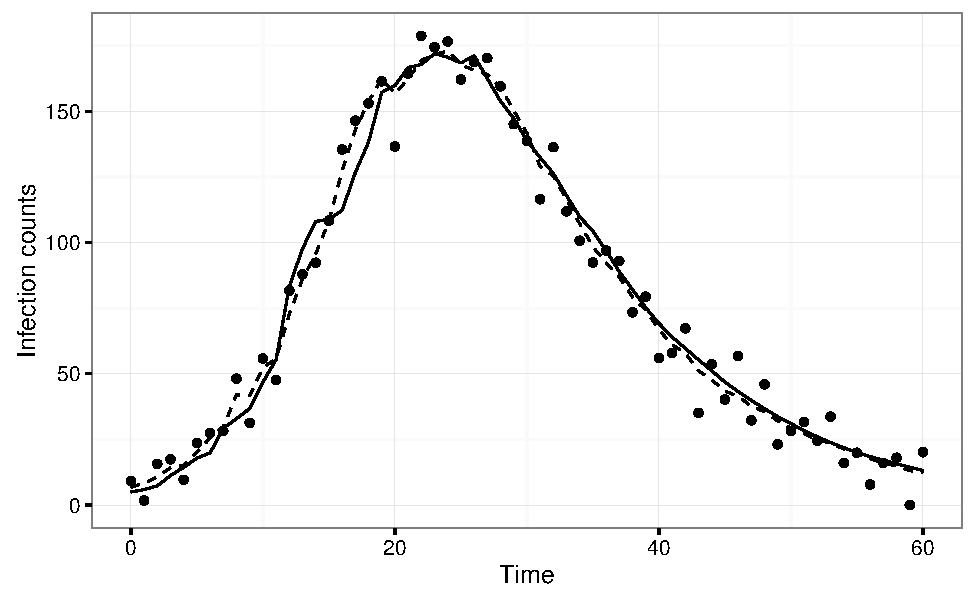
\includegraphics[width=\textwidth,height=\textheight,keepaspectratio=true]{../../writing/SC1/images/if2state}
	\vfill

\end{frame}

\setbeamercolor{normal text}{fg=Grey, bg=white}
\usebeamercolor[fg]{normal text}
\begin{frame}

	\null
	\vfill
	IF2 parameter estimation kernels sample \\
	\vspace{\baselineskip}
	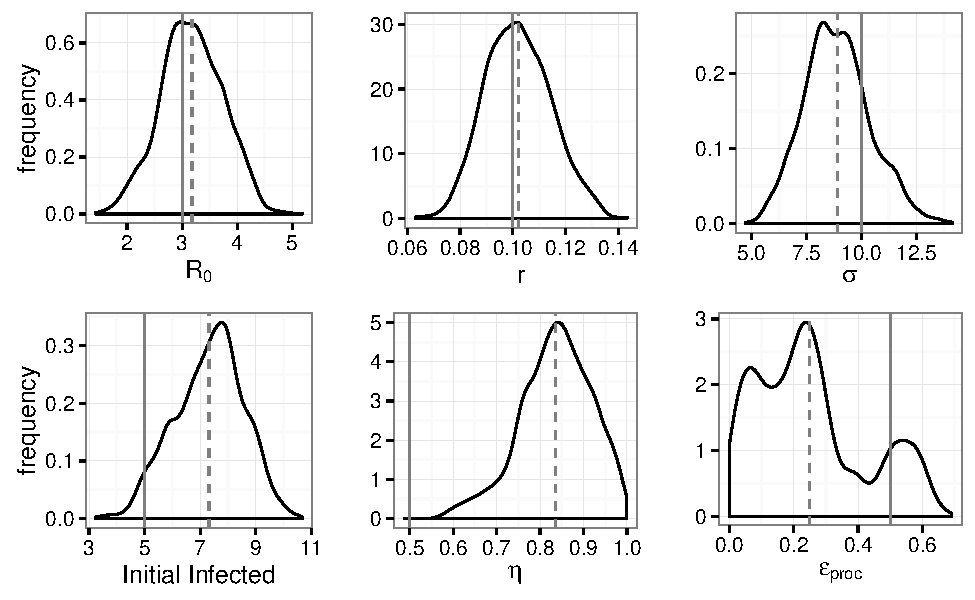
\includegraphics[width=\textwidth,height=\textheight,keepaspectratio=true]{../../writing/SC1/images/if2kernels}
	\vfill

\end{frame}


%%------------------------------------------
%%------------------------------------------

\setbeamercolor{normal text}{fg=Grey, bg=white}
\usebeamercolor[fg]{normal text}
\begin{frame}

	\null
	\vfill
	Mean parameter estimation distributions \\
	\vspace{\baselineskip}
	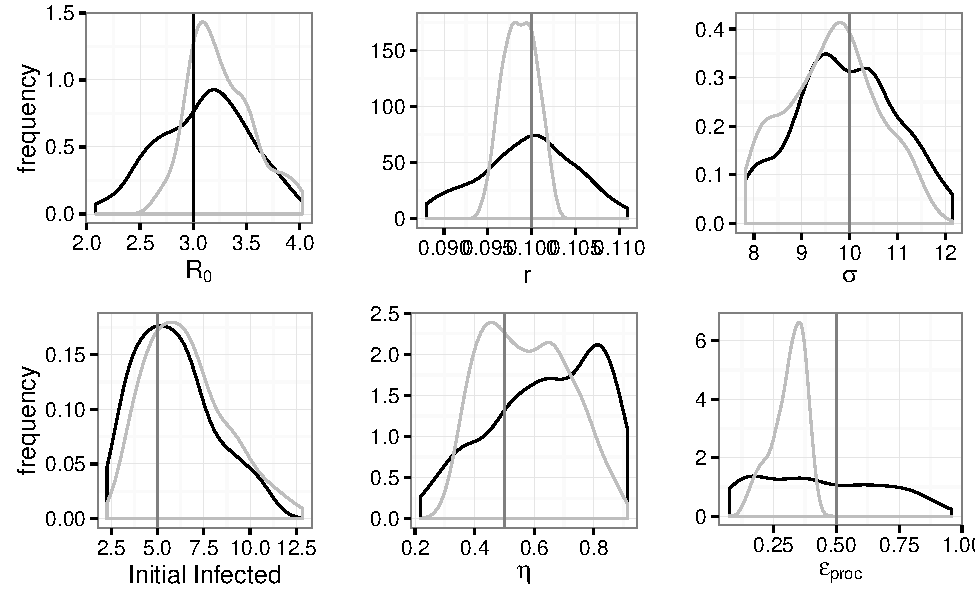
\includegraphics[width=\textwidth,height=\textheight,keepaspectratio=true]{../../writing/SC1/images/combined-multi} \\
	\centering
	\textbf{IF2 \quad \textcolor{Grey50}{HMCMC}}
	\vfill

\end{frame}

\setbeamercolor{normal text}{fg=Grey, bg=white}
\usebeamercolor[fg]{normal text}
\begin{frame}

	\null
	\vfill
	Running times \\
	\vspace{\baselineskip}
	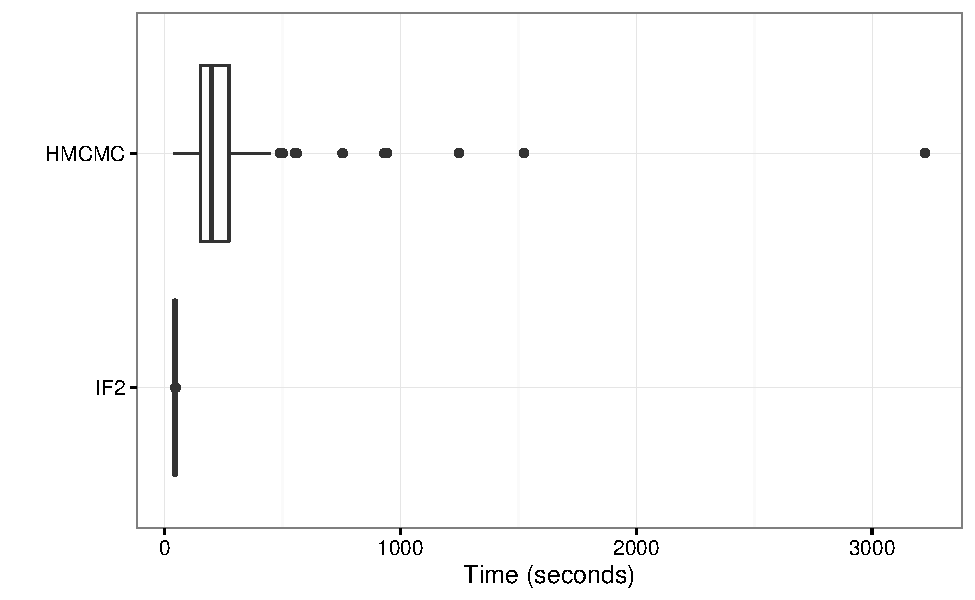
\includegraphics[width=\textwidth,height=\textheight,keepaspectratio=true]{../../writing/SC1/images/timeplot}
	\vfill

\end{frame}

%%------------------------------------------
%%------------------------------------------


%% 5. Forecasting Frameworks
%% --------------------------------------------------------------------------------------
%% --------------------------------------------------------------------------------------

% Section title
\setbeamercolor{normal text}{fg=white, bg=Cyan}
\usebeamercolor[fg]{normal text}
\begin{frame}

	\vspace{2cm}
	\hspace{1cm} {\Huge Forecasting } \\
	\hspace{1cm} {\Huge Frameworks }
	\begin{tikzpicture}[overlay]
	    \node[at=(current page.center), shift={(-4 cm, -4.3 cm)}, opacity=0.25] {
	    	\fontsize{200pt}{0pt}\selectfont
	        \color{white}{5}
	    };
	\end{tikzpicture}

\end{frame}

\setbeamercolor{normal text}{fg=Grey, bg=white}
\usebeamercolor[fg]{normal text}
\begin{frame}

	\begin{columns}
		\begin{column}{0.65\textwidth}

			\large
			IF2 $+$ \\
			Parametric bootstrapping $+$ \\
			Forward simulation
			\vspace{\baselineskip}
			\footnotesize

			\begin{itemize}
				\item Provides additional samples from posterior distribution
				\item Forward simulation using states point estimate, posterior samples
			\end{itemize}
			
			
		\end{column}
		\begin{column}{0.35\textwidth}

			\tiny
			\begin{algorithm}[H]

		        \BlankLine

		        \SetKwInOut{Input}{Input}
		        \SetKwInOut{Output}{Output}
		        \DontPrintSemicolon

		        \Input{Forward simulator $S(\theta)$, data set D}

		        \BlankLine

		        \tcc{Initial fit}
		        $\theta^* \gets IF2(D)$

		        \BlankLine

		        \tcc{Generate artificial data sets}
		        \For{$i = 1:M$}{
			        $D_i \gets S(\theta^*)$
		        }

		        \BlankLine

		        \tcc{Fit to new data sets}
		        \For{$i = 1:M$}{
			        $\theta_i \gets IF2(D_i)$
		        }

		        \tcc{Simulate forward to produce forecasts}
		        \For{$i = 1:M$}{
			        $F_i \gets S(D, \theta_i)$
		        }

		        \BlankLine

		        \Output{Forecast trajectories $F_1, F_2, ..., F_M$}

		        %\caption{Parametric Bootstrap \label{paraboot}}

		    \end{algorithm}

		\end{column}
	\end{columns}

\end{frame}

\setbeamercolor{normal text}{fg=Grey, bg=white}
\usebeamercolor[fg]{normal text}
\begin{frame}

	\null
	\vfill
	IF2 parametric bootstrapping forecast \\
	\vspace{\baselineskip}
	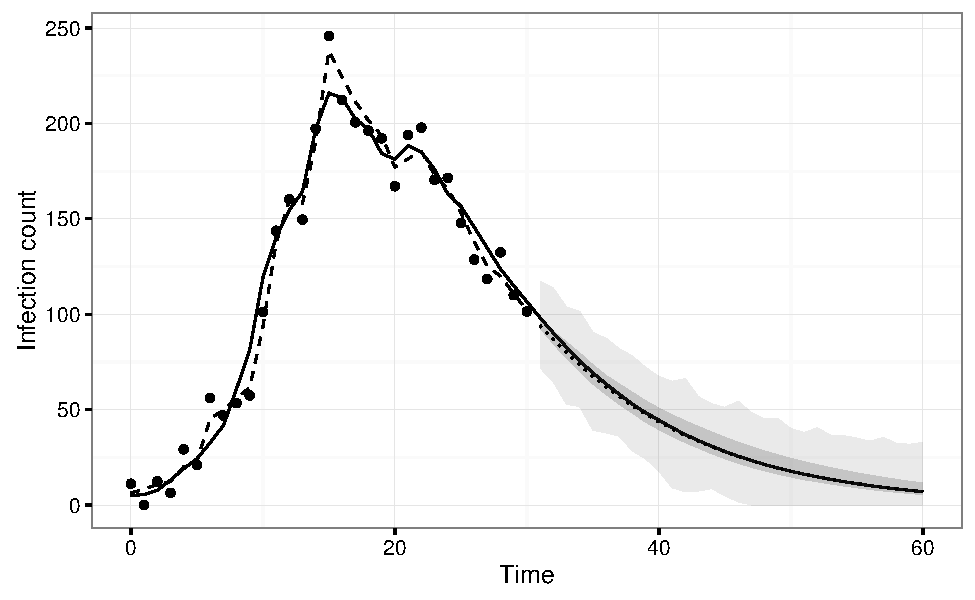
\includegraphics[width=\textwidth,height=\textheight,keepaspectratio=true]{../../writing/SC2/images/if2combined}
	\vfill

\end{frame}

\setbeamercolor{normal text}{fg=Grey, bg=white}
\usebeamercolor[fg]{normal text}
\begin{frame}

	\begin{columns}
		\begin{column}{0.6\textwidth}

			\large
			HMCMC $+$ \\
			State reconstructions $+$ \\
			\vspace{0.35\baselineskip}
			Forward simulation
			\vspace{\baselineskip}
			\footnotesize

			\begin{itemize}
				\item Reconstruct states using latent process noise samples
				\item Simulate forward
			\end{itemize}
			
		\end{column}
		\begin{column}{0.4\textwidth}

			\tiny
			\begin{algorithm}[H]

		        \BlankLine

		        \SetKwInOut{Input}{Input}
		        \SetKwInOut{Output}{Output}
		        \DontPrintSemicolon

		        \tcc{Sample from the posterior}
		        \Input{Posterior samples $\theta_1, \theta_2, ..., \theta_M$}

		        \BlankLine\

		        \tcc{Reconstruct state estimates}
		        \For{$i = 1:M$}{
			        $D_i \gets S(\theta_i)$
		        }

		        \BlankLine

		        \tcc{Simulate forward to produce forecasts}
		        \For{$i = 1:M$}{
			        $F_i \gets S(D_i, \theta_i)$
		        }

		        \BlankLine

		        \Output{Forecast trajectories $F_1, F_2, ..., F_M$}

		        %\caption{Parametric Bootstrap \label{paraboot}}

		    \end{algorithm}

		\end{column}
	\end{columns}

\end{frame}

\setbeamercolor{normal text}{fg=Grey, bg=white}
\usebeamercolor[fg]{normal text}
\begin{frame}

	\null
	\vfill
	HMCMC parametric bootstrapping forecast \\
	\vspace{\baselineskip}
	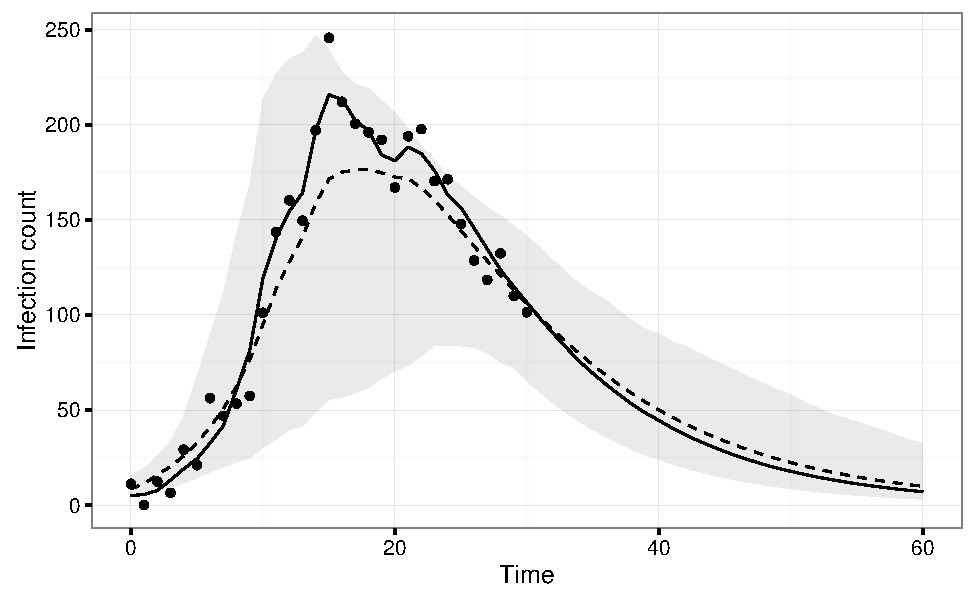
\includegraphics[width=\textwidth,height=\textheight,keepaspectratio=true]{../../writing/SC2/images/hmcforecast}
	\vfill

\end{frame}

\setbeamercolor{normal text}{fg=Grey, bg=white}
\usebeamercolor[fg]{normal text}
\begin{frame}

	\null
	\vfill
	Forecast accuracy comparison \\
	\vspace{\baselineskip}
	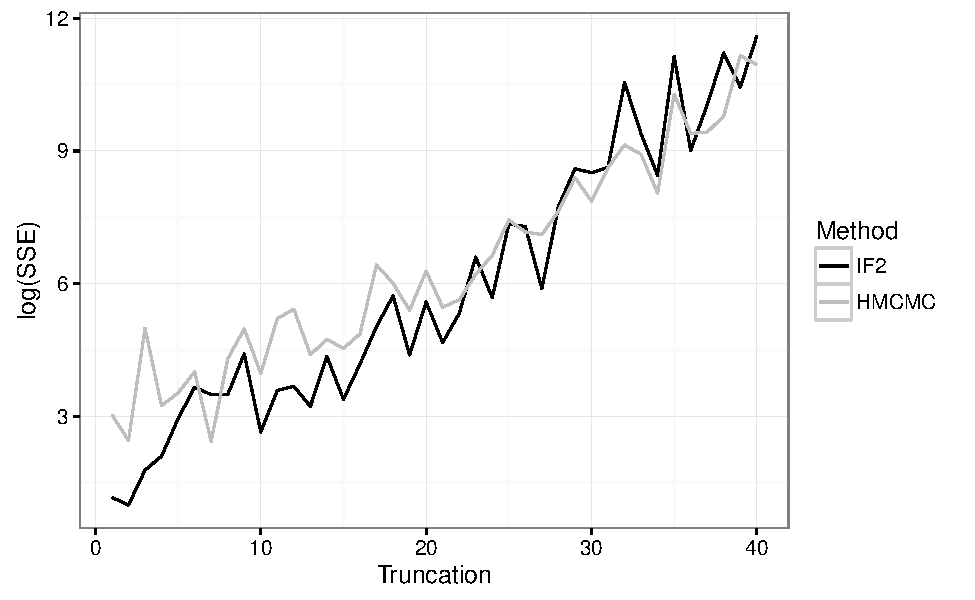
\includegraphics[width=\textwidth,height=\textheight,keepaspectratio=true]{../../writing/SC2/images/truncation}
	\vfill

\end{frame}


%% 6. S-maps and SIRS
%% --------------------------------------------------------------------------------------
%% --------------------------------------------------------------------------------------

% Section title
\setbeamercolor{normal text}{fg=white, bg=Indigo}
\usebeamercolor[fg]{normal text}
\begin{frame}

	\vspace{2cm}
	\hspace{-0.5cm} {\Huge S-maps \& } \\
	%\vspace{0.05cm}
	\hspace{-0.5cm} {\Huge Seasonal Outbreaks }
	\begin{tikzpicture}[overlay]
	    \node[at=(current page.center), shift={(-4.7 cm, -4.3 cm)}, opacity=0.25] {
	    	\fontsize{200pt}{0pt}\selectfont
	        \color{white}{6}
	    };
	\end{tikzpicture}

\end{frame}

% SIRS
\setbeamercolor{normal text}{fg=white, bg=Grey}
\setbeamercolor{footline}{parent=normal text}
\usebeamercolor[fg]{normal text}
\begin{frame}

	\null
	{\large \textcolor{Cyan}{Stochastic SIRS model}}
	\vfill

	\centering
	\begin{align*}
		\dfrac{dS}{dt} 	& = - \beta S I + \textcolor{Teal}{\alpha R}\\
		\dfrac{dI}{dt} 	& = \beta S I - \gamma I \\
		\dfrac{dR}{dt} 	& =  \gamma I - \textcolor{Teal}{\alpha R}
	\end{align*}
	\vspace{0.5\baselineskip}
	$+$	\\
	\vspace{1\baselineskip}
	$\beta_{t+1} = \exp \left[ \beta_t + \eta \left( \bar{\beta} - \beta_t \right) + \mathcal{N}(0, \sigma_{\small\text{proc}}) \right]$

\end{frame}

\setbeamercolor{normal text}{fg=Grey, bg=white}
\usebeamercolor[fg]{normal text}
\begin{frame}

	\null
	\vfill
	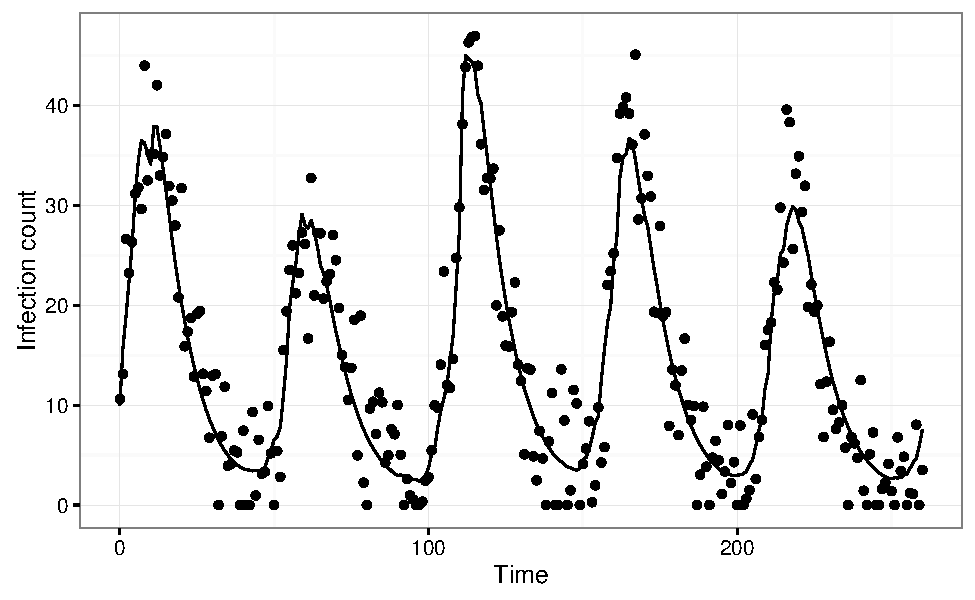
\includegraphics[width=\textwidth,height=\textheight,keepaspectratio=true]{../../writing/SIRS-SMAP/images/dataplot}
	\vfill

\end{frame}

\setbeamercolor{normal text}{fg=Grey, bg=white}
\usebeamercolor[fg]{normal text}
\begin{frame}

	\begin{columns}
		\begin{column}{0.6\textwidth}

			\large
			S-map
			\vspace{\baselineskip}
			\footnotesize

			\begin{itemize}
				\item Construct global mapping of time-lagged vectors (the library) to future states
				\item Weightings are used to penalize poorly matching library vectors
			\end{itemize}
			
		\end{column}
		\begin{column}{0.4\textwidth}

			\tiny
			\begin{algorithm}[H]

		        \BlankLine

		        \SetKwInOut{Input}{Input}
		        \SetKwInOut{Output}{Output}
		        \DontPrintSemicolon

		        \tcc{Select a starting point}
		        \Input{Time series $x_1, x_2, ..., x_T$, embedding dimension $E$, distance penalization $\theta$, forecast length $L$, predictor vector $\mathbf{x_t}$}

		        \BlankLine

		        \tcc{Construct library $\{{\mathbf{x_i}}\}$}
		        \For{$i = E:T$}{
		        	$\mathbf{x_i} = (x_i, x_{i-1}, ...,x_{i-E-1})$
		        }

		        \BlankLine

		        \tcc{Construct mapping from library vectors to predictions}
		        \For{$i = 1:(T_E+1)$}{
		        	\For{$j = 1:E$}{
			        	$A(i,j) = w(||\mathbf{x_i} - \mathbf{x_t}||) \mathbf{x_i}(j)$
			        }
		        }
		        \For{$i = 1:(T_E+1)$}{
			        $b(i) = w(||\mathbf{x_i} - \mathbf{x_t}||) y_i$
		        }

		        \BlankLine

		        \tcc{Use SVD to solve the mapping system, Ac = b}
		        $SVD(Ac = b)$

		        \BlankLine

		        \tcc{Compute forecast}
		        $\hat{y_t} = \sum_{j = 0}^{E} c_t (j) \mathbf{x_t} (j)$

		        \BlankLine

		        \tcc{Forecasted value in time series}
		        \Output{Forecast $\hat{y_t}$}

		        \BlankLine

		        %\caption{S-map \label{smap}}

		    \end{algorithm}

		\end{column}
	\end{columns}

\end{frame}

\setbeamercolor{normal text}{fg=Grey, bg=white}
\usebeamercolor[fg]{normal text}
\begin{frame}

	\null
	\vfill
	S-map forecast \\
	\vspace{\baselineskip}
	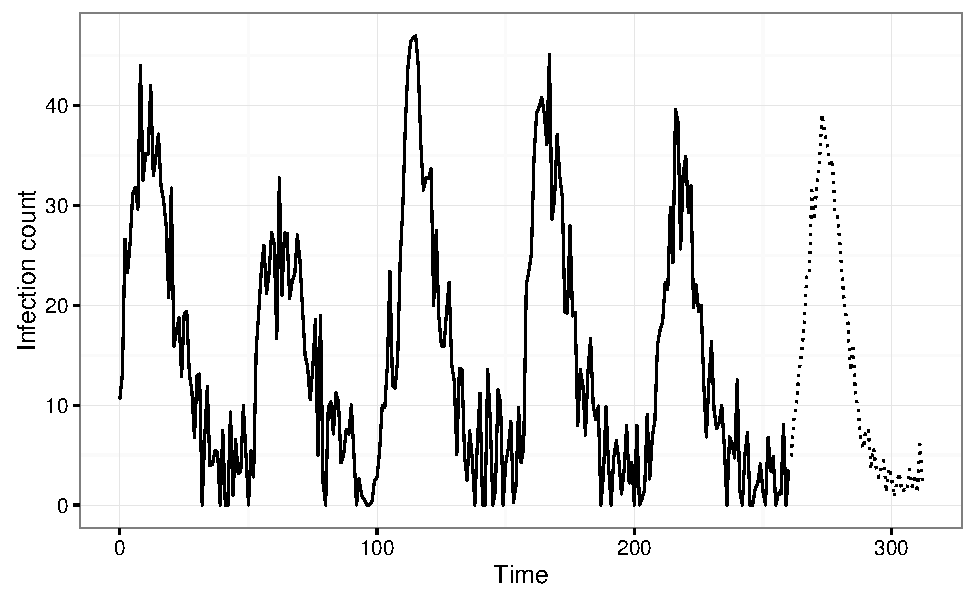
\includegraphics[width=\textwidth,height=\textheight,keepaspectratio=true]{../../writing/SIRS-SMAP/images/smap-project}
	\vfill

\end{frame}

\setbeamercolor{normal text}{fg=Grey, bg=white}
\usebeamercolor[fg]{normal text}
\begin{frame}

	\null
	\vfill
	SIRS model forecasting error \\
	\vspace{\baselineskip}
	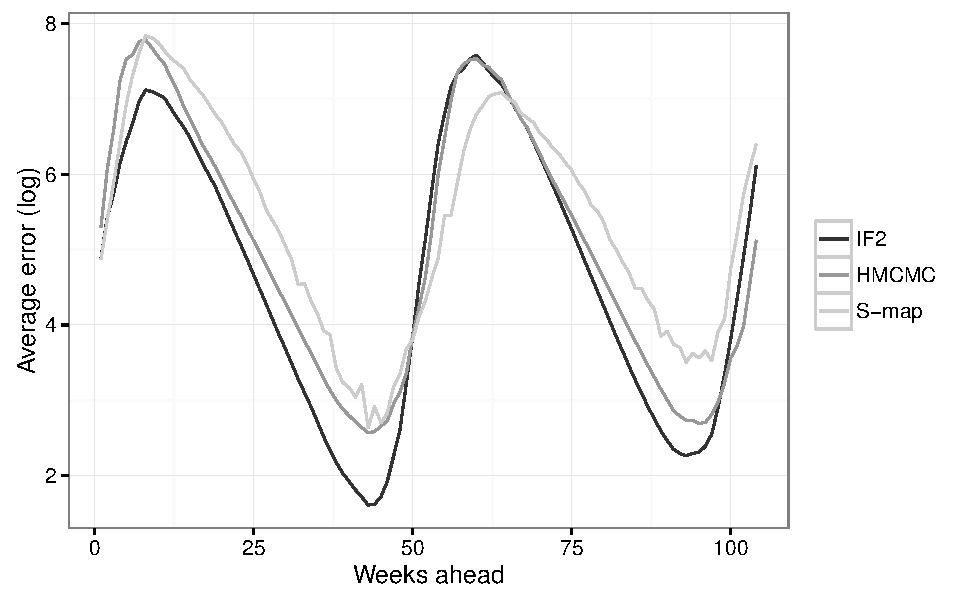
\includegraphics[width=\textwidth,height=\textheight,keepaspectratio=true]{../../writing/SIRS-SMAP/images/sseplot}
	\vfill

\end{frame}

\setbeamercolor{normal text}{fg=Grey, bg=white}
\usebeamercolor[fg]{normal text}
\begin{frame}

	\null
	\vfill
	SIRS model forecasting runtimes \\
	\vspace{\baselineskip}
	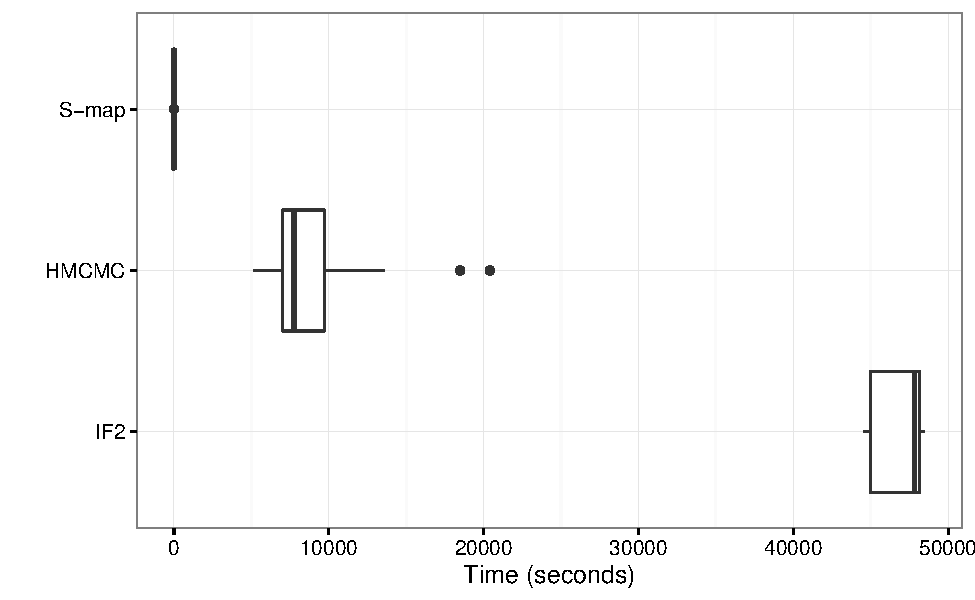
\includegraphics[width=\textwidth,height=\textheight,keepaspectratio=true]{../../writing/SIRS-SMAP/images/timeplot}
	\vfill

	\centering
	\footnotesize
	S-map: 316,000x faster than IF2, 61,800x faster than HMCMC

\end{frame}


%% 7. Spatiotemporal
%% --------------------------------------------------------------------------------------
%% --------------------------------------------------------------------------------------

% Section title
\setbeamercolor{normal text}{fg=white, bg=BlueGrey}
\usebeamercolor[fg]{normal text}
\begin{frame}

	\vspace{2cm}
	\hspace{0cm} {\Huge Spatiotemporal } \\
	\vspace{0.1cm}
	\hspace{0cm} {\Huge Epidemics }
	\begin{tikzpicture}[overlay]
	    \node[at=(current page.center), shift={(-2 cm, -4.2 cm)}, opacity=0.25] {
	    	\fontsize{200pt}{0pt}\selectfont
	        \color{white}{7}
	    };
	\end{tikzpicture}

\end{frame}

\setbeamercolor{normal text}{fg=white, bg=Grey}
\usebeamercolor[fg]{normal text}
\begin{frame}

	\null
	{\large \textcolor{Cyan}{Stochastic Spatial SIR model}}
	\vfill

	\centering
	\begin{align*}
		\dfrac{dS_i}{dt} 	& = - \left(1-\textcolor{Teal}{\phi \frac{M}{M+1}} \right) \beta_i S_i I_i - \textcolor{Teal}{ \frac{\phi}{M+1} } S_i \textcolor{PaleYellow}{\sum_{j = 1}^{M} \beta_{ij}{I_j}} \\
		\dfrac{dI_i}{dt} 	& = \left(1-\textcolor{Teal}{\phi \frac{M}{M+1}} \right) \beta_i S_i I_i + \textcolor{Teal}{ \frac{\phi}{M+1} } S_i \textcolor{PaleYellow}{\sum_{j = 1}^{M} \beta_{ij}{I_j}} - \gamma I_i\\
		\dfrac{dR_i}{dt} 	& = \gamma I_i
	\end{align*}
	\vspace{\baselineskip}
	$+$ \\
	$\beta_{i,t+1} = \exp \left[ \beta_{i,t} + \eta \left( \bar{\beta} - \beta_{i,t} \right) + \mathcal{N}(0, \sigma_{\small\text{proc}}) \right]$

\end{frame}

\setbeamercolor{normal text}{fg=Grey, bg=white}
\usebeamercolor[fg]{normal text}
\begin{frame}

	\null
	\vfill
	Stochastic spatial SIR model simulation (ring topology) \\
	\vspace{\baselineskip}
	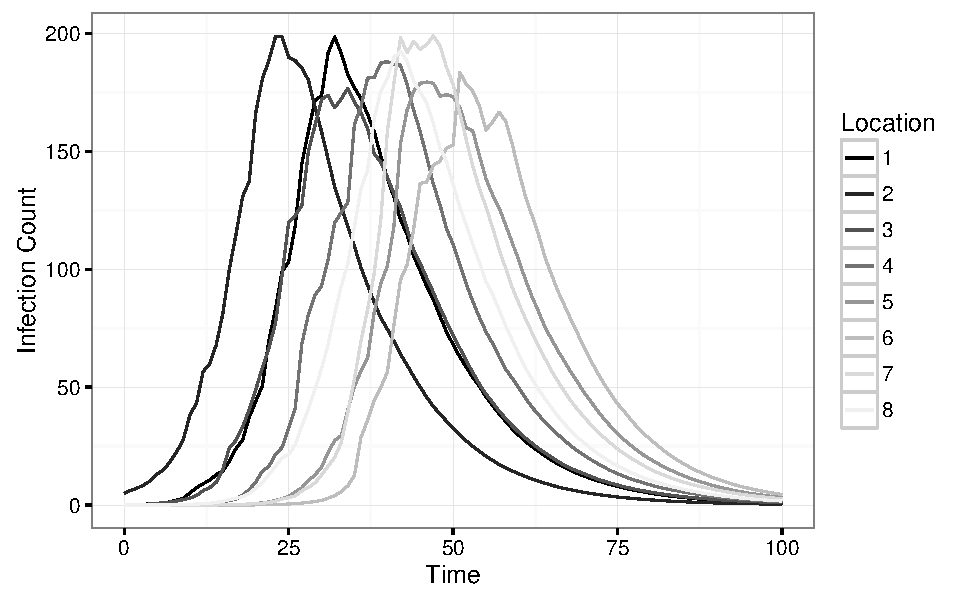
\includegraphics[width=\textwidth,height=\textheight,keepaspectratio=true]{../../writing/SPATIAL/images/dataplot}
	\vfill

\end{frame}

\setbeamercolor{normal text}{fg=Grey, bg=white}
\usebeamercolor[fg]{normal text}
\begin{frame}

	Dewdrop Regression
	\vspace{\baselineskip}

	\begin{itemize}
		\item ``Stitching'' together multiple short time series into single library
		\item Requires scaling
	\end{itemize}

\end{frame}

\setbeamercolor{normal text}{fg=Grey, bg=white}
\usebeamercolor[fg]{normal text}
\begin{frame}

	\null
	\vfill
	Stochastic SIR model forecasting error \\
	\vspace{\baselineskip}
	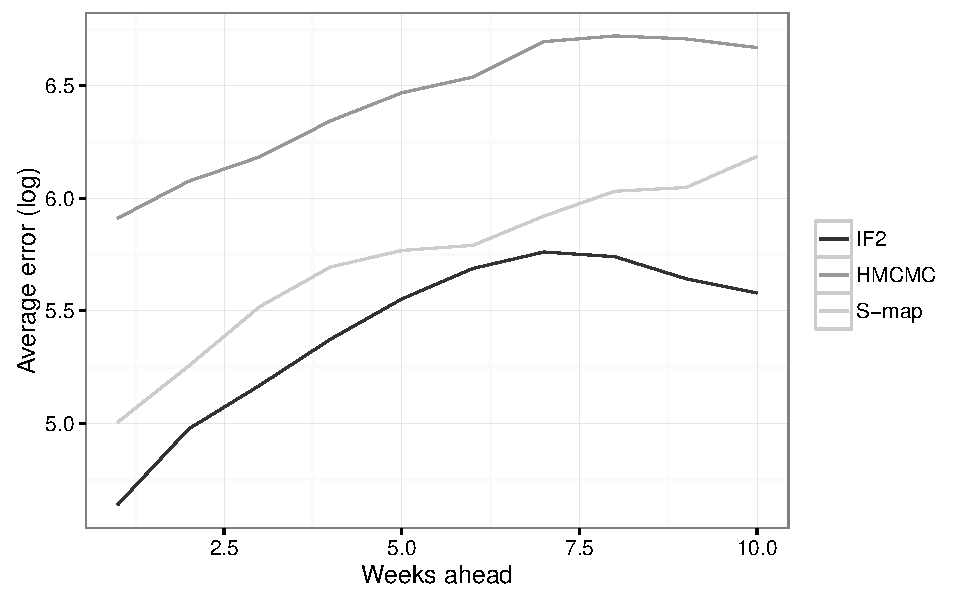
\includegraphics[width=\textwidth,height=\textheight,keepaspectratio=true]{../../writing/SPATIAL/images/sseplot}
	\vfill

\end{frame}

\setbeamercolor{normal text}{fg=Grey, bg=white}
\usebeamercolor[fg]{normal text}
\begin{frame}

	\null
	Spatial SIR model forecasting runtimes \\

	\vfill
	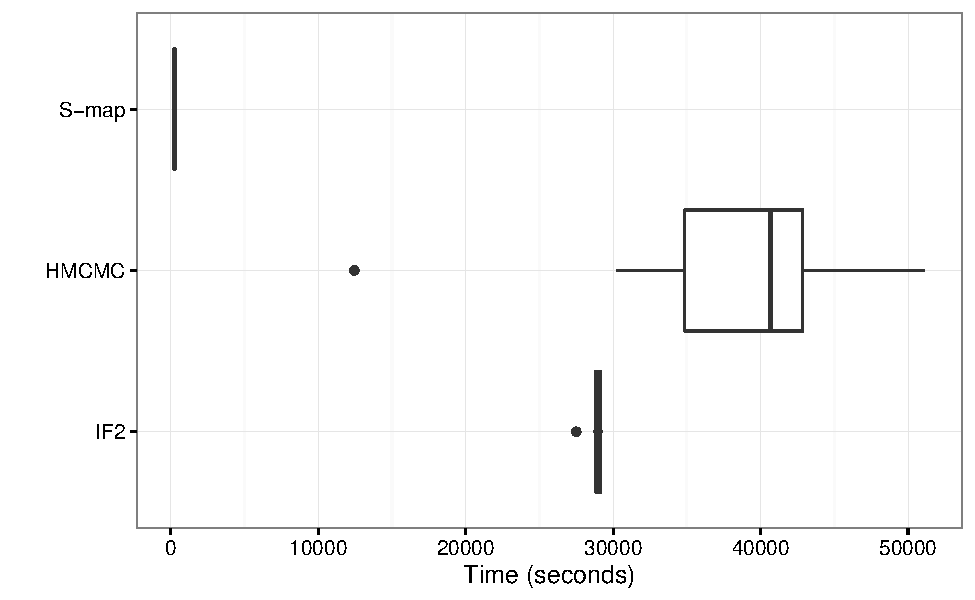
\includegraphics[width=\textwidth,height=\textheight,keepaspectratio=true]{../../writing/SPATIAL/images/timeplot}
	\vfill

\end{frame}

%% 8. Parallelism and Future Directions
%% --------------------------------------------------------------------------------------
%% --------------------------------------------------------------------------------------

% Section title
\setbeamercolor{normal text}{fg=white, bg=DeepOrange}
\usebeamercolor[fg]{normal text}
\begin{frame}

	\vspace{2cm}
	\hspace{0cm} {\Huge Parallelism \& } \\
	\vspace{0.3cm}
	\hspace{0cm} {\Huge Future Directions }
	\begin{tikzpicture}[overlay]
	    \node[at=(current page.center), shift={(-4.7 cm, -4.3 cm)}, opacity=0.25] {
	    	\fontsize{200pt}{0pt}\selectfont
	        \color{white}{8}
	    };
	\end{tikzpicture}

\end{frame}

\setbeamercolor{normal text}{fg=Grey, bg=white}
\usebeamercolor[fg]{normal text}
\begin{frame}

	Conclusions
	\vspace{\baselineskip}

	\begin{itemize}
		\item IF2 produces superior forecasts in all scenarios
		\item S-mapping runs orders of magnitude faster than other methods
	\end{itemize}

\end{frame}

\setbeamercolor{normal text}{fg=Grey, bg=white}
\usebeamercolor[fg]{normal text}
\begin{frame}

	More than Moore
	\vspace{\baselineskip}

	\begin{itemize}
		\item Moore's Law is ceasing to hold
		\item Focus now on distributed computing
		\item MCMC-based methods are resistant to parallelization
		\begin{itemize}
		 	\item Chain construction \textit{requires} iterative dependence
		\end{itemize} 
		\item IF2 exhibits high parallel potential
		\begin{itemize}
			\item Preliminary CUDA (GPU-accelerated) implementation - \texttt{cuIF2}
		\end{itemize}
	\end{itemize}

\end{frame}

\setbeamercolor{normal text}{fg=Grey, bg=white}
\usebeamercolor[fg]{normal text}
\begin{frame}

	\null
	Spatial SIR model fitting times

	\vfill
	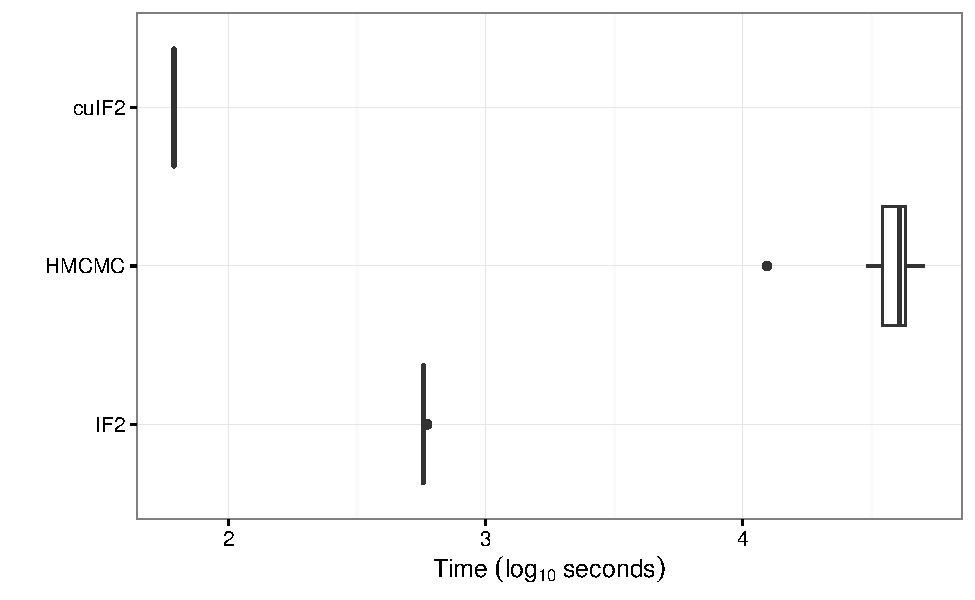
\includegraphics[width=\textwidth,height=\textheight,keepaspectratio=true]{../../writing/SPATIAL/images/timeplot2}
	\vfill

	\centering
	\footnotesize
	\texttt{cuIF2}: 9.33x faster than IF2, 617x faster than HMCMC

\end{frame}

\setbeamercolor{normal text}{fg=Grey, bg=white}
\usebeamercolor[fg]{normal text}
\begin{frame}

	\null
	\vfill
	
\includegraphics[width=\textwidth,height=\textheight,keepaspectratio=true]{images/thesis_defense}
	\vfill

\end{frame}


\end{document}